\documentclass[11pt]{article}
\usepackage[utf8]{inputenc} % Para caracteres en espa�ol
\usepackage{amsmath,amsthm,amsfonts,amssymb,amscd}
\usepackage{multirow,booktabs}
\usepackage[table]{xcolor}
\usepackage{fullpage}
\usepackage{lastpage}
\usepackage{enumitem}
\usepackage{multicol}
\usepackage{fancyhdr}
\usepackage{mathrsfs}
\usepackage{wrapfig}
\usepackage{setspace}
\usepackage{esvect}
\usepackage{calc}
\usepackage{multicol}
\usepackage{cancel}
\usepackage{graphicx}
\graphicspath{ {pictures/} }
\usepackage[retainorgcmds]{IEEEtrantools}
\usepackage[margin=3cm]{geometry}
\usepackage{amsmath}
\newlength{\tabcont}
\setlength{\parindent}{0.0in}
\setlength{\parskip}{0.05in}
\usepackage{empheq}
\usepackage{framed}
\usepackage[most]{tcolorbox}
\usepackage{xcolor}
\colorlet{shadecolor}{orange!15}
\parindent 0in
\parskip 12pt
\geometry{margin=1in, headsep=0.25in}
\theoremstyle{definition}
\newtheorem{defn}{Definition}
\newtheorem{reg}{Rule}
\newtheorem{exer}{Exercise}
\newtheorem{note}{Note}
\newcommand{\volume}{{\ooalign{\hfil$V$\hfil\cr\kern0.08em--\hfil\cr}}}
\newcommand{\parr}{\mathbin{\|}} % Parralel Symbol
\begin{document}
\setcounter{section}{1}
\setcounter{page}{16}
\setcounter{equation}{23}
%\definecolor{babyblue}{rgb}{0.54, 0.81, 0.94}
\definecolor{babyblueeyes}{rgb}{0.63, 0.79, 0.95}
\definecolor{babyblue}{rgb}{0.69, 0.88, 0.9}

 \pagestyle{fancy}
\fancyhf{}
\rhead{Section 3: Electrical Conductivity}
\rfoot{Page \thepage}
\thispagestyle{empty}


\begin{center}
{\LARGE \bf Section 3: Electrical Conductivity}\\
{\large AE435}\\
Spring 2018
\end{center}
\vspace{5mm}
\section{Effect of Collisions}
Here, now particles still feel electric and magnetic body forces, but
the presence of other particles (collisions) is included in the
equation of motion. We initially include the pressure tensor
(thermal particle motion), but neglect it in our derivation of steady-state
scalar conductivity. 

\begin{center}
\vspace{25mm}
\end{center}
\tableofcontents
\newpage
\subsection{No B-Field}
An individual particle has its momentum modified by
collisions. Difficult to track each particle and every
collision in practical situations (although particle-in-cell
models do this, to a certain extent, with macroparticles).

\begin{center}
\vspace{50mm}
\textbf{Figure 4}
\end{center}

Instead, we model collisions as a drag force countering $q \, \vv{E}$
on a swarm of particles. We are considering the mean
motion of a large number of particles, wherein the
integrated effect of many such collisions may be
represented as a damping effect ("drag") on the swarm
motion. This results in the
\begin{shaded}
\textbf{Swarm Equation of Motion:}
\begin{equation}
\begin{aligned}
\frac{\partial}{\partial t} \, n_i \, m_i \, <\vv{v}_i> = n_i \, q_i \, \vv{E} - 	\nu_c \, n_i \, m_i \,<\vv{v}_i> - \nabla P_i
\end{aligned}
\end{equation}
Where 
\begin{equation*}
\begin{split}
<\vv{v}_i> = \text{Swarm Average Velocity for Species } i
\end{split}
\end{equation*}
The terms in this equation are:
\begin{equation*}
\begin{split}
\frac{\partial}{\partial t} \, n_i \, m_i \, <\vv{v}_i>   \qquad &=  \qquad \text{Time rate of change of swarm momentum} \\ \\
n_i \, q_i \, \vv{E}  \qquad &=  \qquad \text{Electrical force on the swarm} \\ \\
\nu_c \, n_i \, m_i \,<\vv{v}_i>   \qquad &=  \qquad \text{"force" due to collisions} \\ \\
\nabla P_i   \qquad &= \qquad \text{Pressure tensor} \\ \\
\end{split}
\end{equation*}
\end{shaded}
\newpage
We have a new term here, $\nu_c$
\begin{shaded}
\textbf{Effective Collision Frequency:}
\begin{equation}
\begin{aligned}
\nu_c = \sum n_j \, Q_j^{(P)} \, <|\vv{v}_j|>
\end{aligned}
\end{equation}
Defined by its effect on swarm momentum.

Where
\begin{equation*}
\begin{split}
Q_j^{(P)} &= \text{Momentum transfer cross-section} \\ \\
 <|\vv{v}_j|> & = \text{Mean relative speed between charge carrier species} j \text{and what its colliding with.} 
\end{split}
\end{equation*}
\end{shaded}
Turns out to be hard to estimate all the terms that make up
so usually treat the collision frequency as an empirical
parameter.

If we ignore effects that change the number density of a
species (ionization, recombination, charge-exchange, etc.)
the momentum equation for species i above becomes:
\begin{equation}
\begin{aligned}
m_i \, n_i \,  \frac{\partial}{\partial t} \, <\vv{v}_i> = n_i \, q_i \, \vv{E} - 	\nu_c \, n_i \, m_i \,<\vv{v}_i> - \nabla P_i
\end{aligned}
\end{equation}
Switching from Langrangian to Eulerian system
(Lagrangian - tracking individual particle/fluid packets vs.
time as move through flowfield, Eulerian - tracking how
the flowfield properties change with time)
\begin{equation}
\begin{aligned}
m_i \, n_i \, \bigg[ \frac{\partial <\vv{v}_i>}{\partial t} + <\vv{v}_i> \cdot \nabla <\vv{v}_i> \bigg] = n_i \, q_i \, \vv{E} - 	\nu_c \, n_i \, m_i \,<\vv{v}_i> - \nabla P_i
\end{aligned}
\end{equation}
For now, we can neglect the pressure tensor $\nabla P_i$. For
constant $\nu_c$, independent of $<\vv{v}_i>$, we get the...
\begin{shaded}
\textbf{Swarm Velocity Equation:}
\begin{equation}
\begin{aligned}
<\vv{v}> = \frac{q}{m \, \nu_c} \vv{E} + \vv{c} \, e^{-\nu_c \, t}
\end{aligned}
\end{equation}
Where
\begin{equation*}
\begin{split}
\frac{q}{m \, \nu_c} \vv{E} &= \text{Steady-state solution} \\ \\
\vv{c} \, e^{-\nu_c \, t} &= \text{Transient response}
\end{split}
\end{equation*}
Note: This equation only applies when we neglect the pressure tensor and assume constant effective collision frequency, $\nu_c$.
\end{shaded}
\newpage
Notice how the settling time of the transient response is set by the
collision frequency. After the switching transient has
died away, the \textbf{steady-state current density} becomes:
\begin{equation}
\begin{aligned}
\vv{j} = n \, q \, <\vv{v}> = \frac{n \,q^2}{m \, \nu_c} \vv{E}
\end{aligned}
\end{equation}

Thus the \textbf{Scalar Conductivity in a Steady E-field} is (from $\vv{j} = \sigma \, \vv{E}$):
\begin{subequations}
\begin{equation}
\begin{aligned}
\sigma = \frac{n \,q^2}{m \, \nu_c}
\end{aligned}
\end{equation}

and the \textbf{Plasma Frequency}, $\omega_P$ is defined:
\begin{equation}
\begin{aligned}
\omega_{P_{\pm}}^2 =  \frac{n_{\pm} \,q_{\pm}^2}{m_{\pm} \, \epsilon_o}
\end{aligned}
\end{equation}

Such that the scalar conductivity of a steady E-field becomes:
\begin{equation}
\begin{aligned}
\sigma = \epsilon_o \frac{\omega_{P_{\pm}}^2}{\nu_c}
\end{aligned}
\end{equation}
\end{subequations}
\newpage
\subsection{Steady B-Field}
We know that without collisions, particles will undergo an
ExB drift. No charge separation, so no conduction, and
drift velocity is:
\begin{equation*}
\begin{aligned}
\vv{v}_i = \frac{\vv{E} \times \vv{B}}{B^2} = \vv{v}_e
\end{aligned}
\end{equation*}
To determine the effect of magnetic field, the relationship
between the gyro/cyclotron frequency, $\omega_B$, and
collision frequency, $\nu_c$, is key. Thus we define the...
\begin{shaded}
\textbf{Hall Parameter:}
\begin{equation}
\begin{aligned}
\Omega = \frac{\omega_B}{\nu_c}
\end{aligned}
\end{equation}
\end{shaded}

\textbf{Why do we care about conductivity?}

We care about current flow because in a lot of electric propulsion systems, there is current flowing through the plasma propellant. That current creates a magnetic field which interacts with other magnetic fields present. Often times we are expelling a current of charged particles and we want to see the how that current is conducted through the gas.

So when we add in magnetic field, we are really interested in the relationship between the frequency of that gyration and the frequency that they are having their collisions. 

\textbf{How is Hall parameter related to electrical conductivity?}
\newpage
\large{\textbf{Case 1: }Small Hall Parameter}
\begin{equation*}
\begin{aligned}
\Omega < < 1 \qquad \qquad \nu_c > > \omega_B
\end{aligned}
\end{equation*}
The collision frequency is high compared to the
gyro-frequency. Particles generally don't complete
even part of a gyration before colliding. In this case,
gyro-motion doesn't affect conduction along Efield
very much; the cross-field component of the current is
small. This conductivity is scalar.

\begin{center}
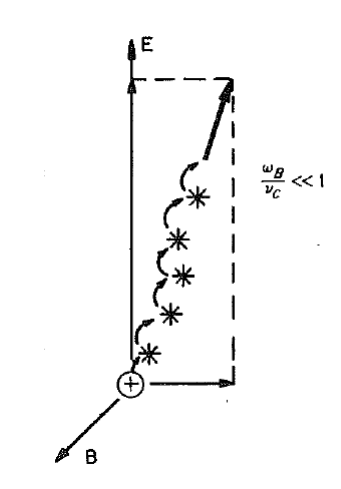
\includegraphics[scale=0.65]{6a.png}
\end{center}

The magnetic field is not having that big of an effect. The particles are trying to complete a gyro-motion but before they can go around in an entire circle, they have a collision. Its almost as if the magnetic field isn't even there. Its the electric field trying to drive the particles in a certain direction. Basically the same conductivity we seen in Equation 30.
\newpage
\textbf{Case 2: }Large Hall Parameter
\begin{equation*}
\begin{aligned}
\Omega > > 1 \qquad \qquad \nu_c < < \omega_B
\end{aligned}
\end{equation*}
If the collision frequency is low compared to the
gyro-frequency, particles generally complete many
gyrations before colliding. In this case the cross-field
component of the current is large, and the conductivity is
tensor.

\begin{center}
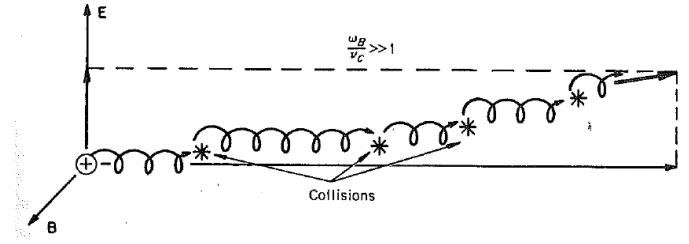
\includegraphics[scale=0.65]{6b.png}
\end{center}

What we are seeing here then is that the particles are completing lots of gyrations and drifting in the ExB direction before collisions. After a collision, the particle moves upwards because the electric field is pointing up. This is why, in general, the conductivity, $\sigma$, is written as a tensor: we can have anisotropic effects.
\newpage
\textbf{Case 3: }Hall Parameter of 1
\begin{equation*}
\begin{aligned}
\Omega \approx 1 \qquad \qquad \nu_c \approx \omega_B
\end{aligned}
\end{equation*}
If the collision frequency is close to the
gyro-frequency, particles generally complete a partial
gyration before colliding, then moving in the direction of the E-field. In this intermediate case,
we can divide the current into:
\begin{itemize}
\item Scalar conduction current parallel to E, \quad  $\vv{j}_{||} \, || \, \vv{E}$
\item Hall current perpendicular to E, \quad $\vv{j}_{\perp} \, \perp \, \vv{E}$
\end{itemize}

\begin{center}
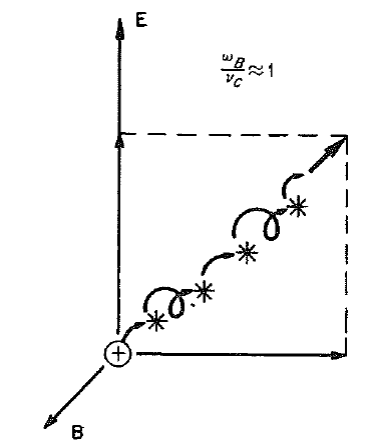
\includegraphics[scale=0.65]{6c.png}
\end{center}

\newpage

We started this section off by talking about the ExB drift. The positive and negative charges drift with the same speed $\frac{E}{B}$. 

\textbf{Question: }Does this mean that we can never get a Hall current, a current perpendicular to E and B for two species (Positive Ions and Negative Electrons
)? 

\textbf{Answer: }No, it doesn't. We can get a Hall current for two species because one of them can be magnetized and have a large Hall Parameter where as the other may not be magnetized and have a small Hall Parameter.

So we can imagine a case (with a figure similar to the one in Case 3) where the ions (a positive species) are not magnetized and only moving up the page in the E direction but the electrons (a negative species) are magnetized and they have motion in the ExB direction generating a Hall Current. Even if there are two species, it is possible to have them both have different hall parameters and as a result, have a Hall Current.

This is not uncommon to have different Hall parameters for different species.
Typically:

\begin{equation}
\begin{aligned}
\Omega_{e^{-}} > > \Omega_{\text{ion}}
\end{aligned}
\end{equation}

so, electrons are "trapped" on the B-field lines, while ions are not affected by B. This is a design criterion for Hall
thrusters (where we want the electrons to be impeded by B-field, but not the ions), and is also the case inside the discharge chamber of ion engines.

\newpage
\end{document}